\documentclass[serif, aspectratio=169]{beamer}
%\documentclass[serif]{beamer}  % for 4:3 ratio

\RequirePackage{minted2}
\usepackage[T1]{fontenc} 
\usepackage[utf8]{inputenc}
\usepackage{fourier} % see "http://faq.ktug.org/wiki/uploads/MathFonts.pdf" for other options
\usepackage{hyperref}
\usepackage{latexsym,amsmath,xcolor,multicol,booktabs,calligra}
\usepackage{graphicx,pstricks,listings,stackengine}
\usepackage{lipsum}
\usepackage{../../../TEMPLATES/template_style}

%imports customs%
\usepackage{caption}    % for subfigures
\usepackage{subcaption} % for subfigures
\usepackage{ragged2e}
\usepackage{booktabs,makecell}
\usepackage{colortbl}
\usepackage{multirow}
\usepackage{cite}
\usepackage{tcolorbox}
\usepackage[sort,authoryear]{natbib}

\author{Julien Bezançon}

\title{Python Programmation}
\subtitle{CM 6~: Python Libraries}

\institute{julien.bezancon@univ-lorraine.fr / \url{https://julienbez.github.io}}

\date{}

% defs
\def\cmd#1{\texttt{\color{red}\footnotesize $\backslash$#1}}
\def\env#1{\texttt{\color{blue}\footnotesize #1}}

% set colors
\definecolor{hkustyellow}{RGB}{167, 131, 55}
\definecolor{hkustblue}{RGB}{0, 56, 116}
\definecolor{hkustred}{RGB}{209, 51, 59}

\lstset{
    basicstyle=\ttfamily\small,
    keywordstyle=\bfseries\color{deepblue},
    emphstyle=\ttfamily\color{deepred},    % Custom highlighting style
    stringstyle=\color{deepgreen},
    numbers=left,
    numberstyle=\small\color{halfgray},
    rulesepcolor=\color{red!20!green!20!blue!20},
    frame=shadowbox,
}

\begin{document} %  --- --- --- --- --- --- --- --- --- --- --- --- 

\begin{frame}[noframenumbering,plain]
    \titlepage
    \vspace*{-0.6cm}
    \begin{figure}[htpb]
        \begin{center}
            \hspace{0.3cm}
            
\includegraphics[width=0.7\columnwidth]{../../../IMAGES/loria_idmc.png}
        \end{center}
    \end{figure}
\end{frame}

% \begin{frame}    
%     \tableofcontents[sectionstyle=show,
%     subsectionstyle=show/shaded/hide,
%     subsubsectionstyle=show/shaded/hide]
% \end{frame}

\section{Before we start...}

\begin{exoframe}
    \begin{center}
        \Large
        What did you learn during last lecture ? \\
        Any questions ?
    \end{center}
\end{exoframe}

\begin{frame}{Last Lecture Doggy bag}
    \begin{minipage}{0.45\columnwidth}
        \begin{block}{File handling}
            \begin{itemize}
                \item Open and write a file
                \item Encoding and pathing
                \item String parsing
                \item Dedicated libraries
            \end{itemize}
        \end{block}
        \begin{block}{File navigation}
            \begin{itemize}
                \item File VS python structures
                \item Common errors
            \end{itemize}
        \end{block}
    \end{minipage}
    \hfill
    \begin{minipage}{0.45\columnwidth}
        \begin{figure}
            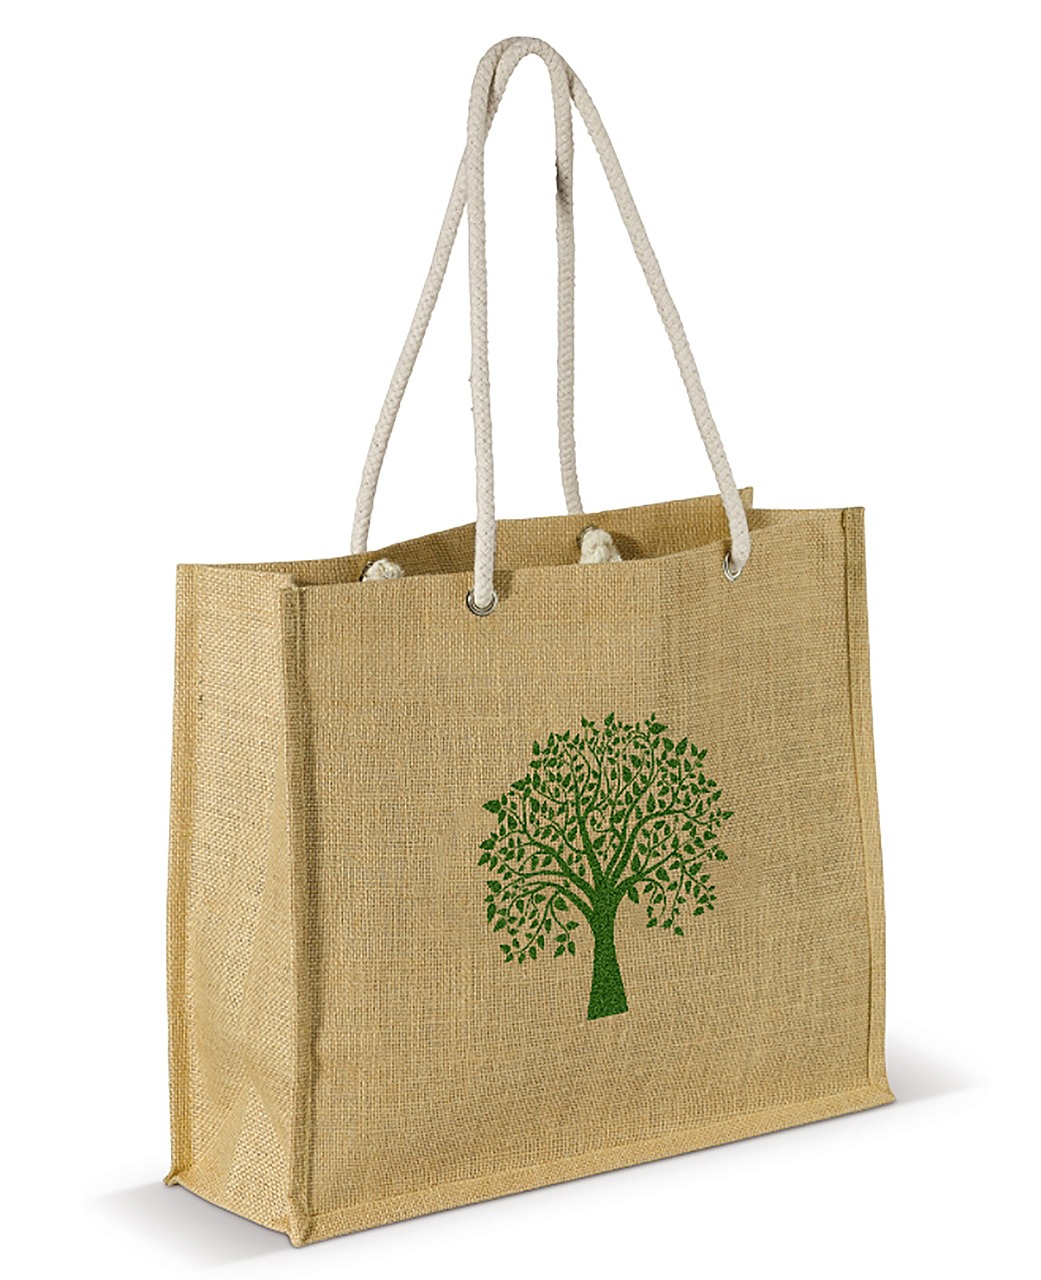
\includegraphics[width=0.9\columnwidth]{../../../FIGURES/divers/doggybag.jpg}
        \end{figure}
    \end{minipage}
\end{frame}

\section{Libraries}

\begin{frame}[fragile]{What is a Library ?}
    \begin{pythoncode}
    import os
    import json
    import glob
    
    import pandas as pd
    from tqdm import tqdm
    \end{pythoncode}
    \vfill
    \begin{block}{Libraries are the toolboxes of Python}
        \begin{itemize}
            \item Contains pre-written code and functions
            \item Can be installed and added freely
            \item Designed for specific usecases
        \end{itemize}
    \end{block}
\end{frame}

\begin{frame}[fragile]{An Example: the "os" Library}
    \begin{pythoncode}
    import os
    
    # some calls from the os Library
    os.walk()
    os.rename()
    os.mkdir()
    os.exit()
    \end{pythoncode}
    \vfill
    \begin{block}{"os" is a standard library}
        \begin{itemize}
            \item Installed by default with Python
            \item Other libraries need to be manually added
        \end{itemize}
    \end{block}
\end{frame}

\begin{frame}[fragile]{Most libraries are not Installed by Default}
    \begin{pythoncode}
    import pandas as pd
    df = pd.read_csv('data.csv')
    \end{pythoncode}
    \vfill
    \begin{CLI}
        $>$ python my\_script.py \\
        Traceback (most recent call last): \\
        ~~File "my\_script.py", line 1, in $<$module$>$ \\
        ~~~~import pandas \\
        ImportError: No module named pandas \\
    \end{CLI}
\end{frame}

\begin{frame}{How to Install a Library}
    \begin{block}{With pip}
        \vspace{5pt}
        \begin{CLI}
            pip install pandas
        \end{CLI}
    \end{block}
    \begin{block}{With uv}
        \vspace{5pt}
        \begin{CLI}
            uv add pandas
        \end{CLI}
    \end{block}
    \begin{block}{With conda}
        \vspace{5pt}
        \begin{CLI}
            conda install pandas
        \end{CLI}
    \end{block}
\end{frame}

\begin{frame}{Installing a List of Libraries}
        \begin{block}{With pip}
        \vspace{5pt}
        \begin{CLI}
            pip install -r requirements.txt
        \end{CLI}
    \end{block}
    \begin{block}{With uv}
        \vspace{5pt}
        \begin{CLI}
            uv add -r requirements.txt
        \end{CLI}
    \end{block}
    \begin{block}{With conda}
        \vspace{5pt}
        \begin{CLI}
            conda create -\nothing{}-file environment.yml
        \end{CLI}
    \end{block}
\end{frame}

\begin{exoframe}{}
    \begin{center}
        \Large
        We will now overview 3 packages. \\
        Download the jupyter-notebooks on Arche.
    \end{center}
\end{exoframe}

\begin{frame}{Packages: Summary}
    \begin{block}{Python has hundred of thousands of packages}
        \begin{itemize}
            \item We will not see them all in this lecture
            \item You will not remember how to use each one of them
        \end{itemize}
    \end{block}
    \begin{block}{Best practices}
        \begin{itemize}
            \item Get used to python package documentation and common usages
            \item Do not hesitate to use forums and search engines \textbf{($\ne$ generative AI !!!)}
        \end{itemize}
    \end{block}
    \vfill
    \begin{center}
        \Large
        You will master Python by developping good habits. \\
        Number one good habit = knowing how to find solutions.
    \end{center}
\end{frame}

\section{Environments}

\begin{frame}{Common Issues in Python}
    \begin{block}{Library versions issues}
        \begin{itemize}
            \item One script needs pandas v2.2.3 and the other needs pandas v3.0.6
            \item You can only have one version of a library
        \end{itemize}
    \end{block}
    \begin{block}{Python versions issues}
        \begin{itemize}
            \item You want to use an old script, but it uses Python 2.7
            \item You can have only one version of Python installed
        \end{itemize}
    \end{block}
    \vfill
    \begin{center}
        \Large
        Solution: create Python virtual environments !
    \end{center}
\end{frame}

\begin{frame}{What is a Python Virtual Environment ?}
    \begin{block}{From W3School\footnote{\url{https://www.w3schools.com/python/python_virtualenv.asp}}}
        \begin{tcolorbox}
        A virtual environment in Python is an isolated environment on your computer, where you can run and test your Python projects.
        \end{tcolorbox}
    \end{block}
    \vfill
    \begin{center}
        \Large
        Python virtual environments (venv) allow you to manage projects \\ 
        which have different Python configurations.
    \end{center}
\end{frame}

\begin{frame}{How does a venv Works ?}
    \begin{figure}
        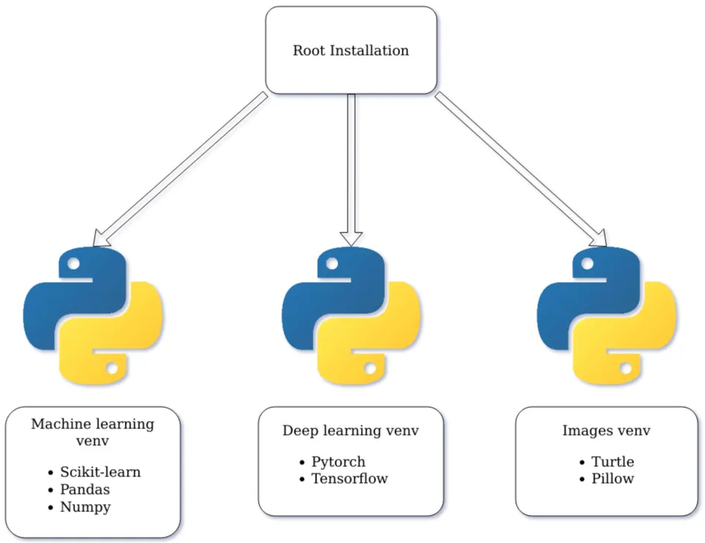
\includegraphics[width=0.55\columnwidth]{../../../FIGURES/python/python_venv.png}
        \caption*{Source: \url{https://www.python-engineer.com/}}
    \end{figure}
\end{frame}

\begin{frame}{Venv Cheatsheet (python + pip)}
    \begin{block}{How to create a venv}
        \vspace{5pt}
        \begin{CLI}
            $>$ python -m venv venv\_name \\
            $>$ source venv\_name/bin/activate \\
        \end{CLI}
    \end{block}
    \begin{block}{How to use jupyter-notebook with this venv}
        \vspace{5pt}
        \begin{CLI}
            $>$ pip install -\nothing{}-user ipykernel \\
            $>$ python -m ipykernel install -\nothing{}-user \\
        \end{CLI}
    \end{block}
\end{frame}

\begin{frame}{Venv Cheatsheet (uv)}
    \begin{block}{How to create a venv}
        \vspace{5pt}
        \begin{CLI}
            $>$ cd my\_project \\ 
            $>$ uv init \\
        \end{CLI}
    \end{block}
    \begin{block}{How to use jupyter-notebook with this venv}
        \vspace{5pt}
        \begin{CLI}
            $>$ uv add jupyter \\ 
            $>$ uv run jupyter notebook \\
        \end{CLI}
    \end{block}
\end{frame}

\begin{frame}{Venv Cheatsheet (conda)}
    \begin{block}{How to create a venv}
        \vspace{5pt}
        \begin{CLI}
            $>$ conda create -\nothing{}-name venv\_name \\
            $>$ conda activate venv\_name \\
        \end{CLI}
    \end{block}
    \begin{block}{How to use jupyter-notebook with this venv}
        \vspace{5pt}
        \begin{CLI}
            $>$ conda install jupyter \\
            $>$ jupyter notebook \\
        \end{CLI}
    \end{block}
\end{frame}

\begin{frame}{Using the Default environment is BAD}
    \begin{block}{Library compatibilities issues}
        \begin{itemize}
            \item Two libraries have common dependencies - but in different versions
            \item You WILL end up re-installing everything
        \end{itemize}
    \end{block}
    \begin{block}{Reproductibility issues}
        \begin{itemize}
            \item You want to upload your code with mandatories libraries
            \item You want to list each library and the version used - as well as their dependencies
        \end{itemize}
    \end{block}
    \vfill
    \begin{center}
        \Large
        Most of the time, you won't even realize there is an issue !
    \end{center}
\end{frame}

\section{Modules}

\begin{frame}[fragile]{What is a Module ?}
    \begin{pythoncode}
    from script_1 import function_1, function_2
    from src.others.script_2 import *
    import script_3
    import script_3 as sc

    function_1()
    function_2()
    script_3.function_3()
    sc.function_3()
    \end{pythoncode}
    \vfill
    \begin{block}{Modules help you to structure your projects}
        \begin{itemize}
            \item They must be a python file (.py extension)
            \item They should only contain functions !
        \end{itemize}
    \end{block}
\end{frame}

\begin{frame}{How to use Modules ?}
    \begin{minipage}{0.40\columnwidth}
        \begin{figure}
            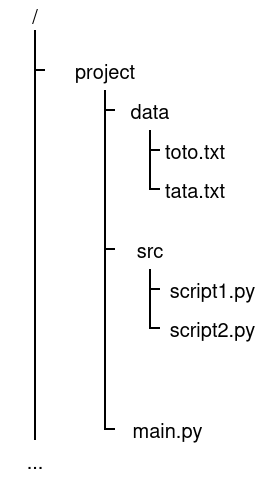
\includegraphics[width=0.7\columnwidth]{../../../FIGURES/python/folder_tree_modules.png}
        \end{figure}
    \end{minipage}
    \hfill
    \begin{minipage}{0.50\columnwidth}
        \begin{block}{Good practices}
            \begin{itemize}
                \item Keep modules short and specific
                \item Place modules in a child folder
                \item Add \wordbox{\_\_init\_\_.py} in said child folder
                \vspace{10pt}
                \item Avoid circular module imports
                \item Import everything in a "main" script
            \end{itemize}
        \end{block}
    \end{minipage}
\end{frame}

\begin{frame}{Some Questions}
    \begin{block}{What happens if...}
        \begin{itemize}
            \item I import script1 in script2 and script2 in script1 ?
            \item I import script1, which contains package imports ?
            \item I import script1, which contains variable names ?
            \vspace{10pt}
            \item I want to access toto.txt from script1 ?
            \item I want to access toto.txt from script1 from main ?
        \end{itemize}
    \end{block}
    \vfill
    \begin{center}
        \Large
        Always be careful with paths when using modules !
    \end{center}
\end{frame}

\begin{frame}{Doggy bag}
    \begin{minipage}{0.45\columnwidth}
        \begin{block}{Libraries}
            \begin{itemize}
                \item The toolboxes of python
                \item pandas, sklearn and matplotlib
            \end{itemize}
        \end{block}
        \begin{block}{Virtual env}
            \begin{itemize}
                \item Use them !
                \item Global venv = BAD
            \end{itemize}
        \end{block}
        \begin{block}{Modules}
            \begin{itemize}
                \item Snippets of code
                \item Better code structure
            \end{itemize}
        \end{block}
    \end{minipage}
    \hfill
    \begin{minipage}{0.45\columnwidth}
        \begin{figure}
            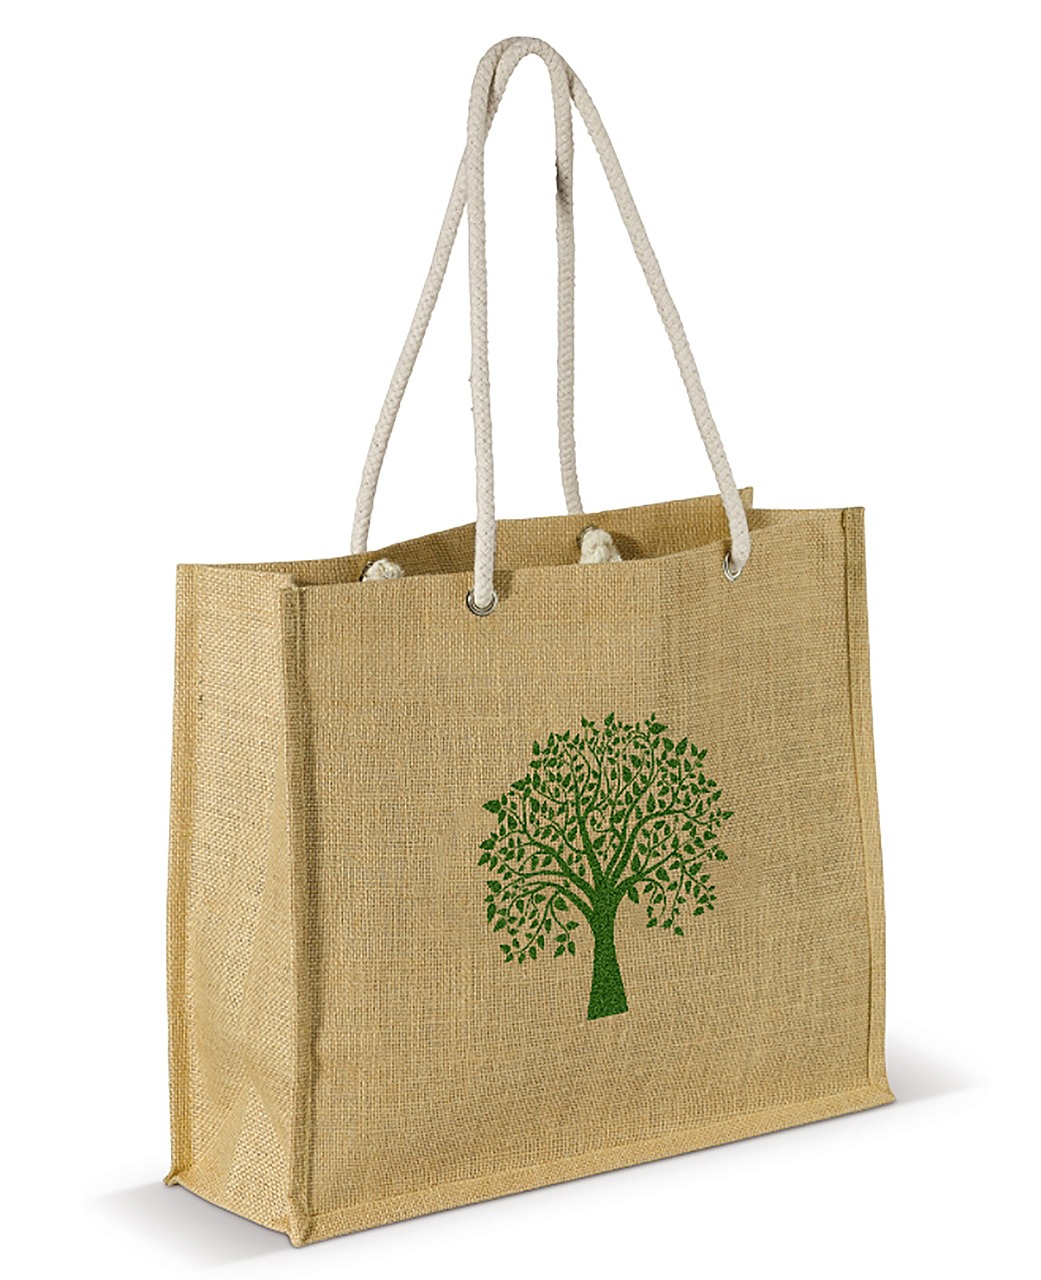
\includegraphics[width=0.9\columnwidth]{../../../FIGURES/divers/doggybag.jpg}
        \end{figure}
    \end{minipage}
\end{frame}

\end{document}
